% Options for packages loaded elsewhere
\PassOptionsToPackage{unicode}{hyperref}
\PassOptionsToPackage{hyphens}{url}
\PassOptionsToPackage{dvipsnames,svgnames,x11names}{xcolor}
%
\documentclass[
  letterpaper,
  DIV=11,
  numbers=noendperiod]{scrartcl}
\usepackage{beamerarticle} % needs to be loaded first

\usepackage{amsmath,amssymb}
\usepackage{iftex}
\ifPDFTeX
  \usepackage[T1]{fontenc}
  \usepackage[utf8]{inputenc}
  \usepackage{textcomp} % provide euro and other symbols
\else % if luatex or xetex
  \usepackage{unicode-math}
  \defaultfontfeatures{Scale=MatchLowercase}
  \defaultfontfeatures[\rmfamily]{Ligatures=TeX,Scale=1}
\fi
\usepackage{lmodern}
\ifPDFTeX\else  
    % xetex/luatex font selection
\fi
% Use upquote if available, for straight quotes in verbatim environments
\IfFileExists{upquote.sty}{\usepackage{upquote}}{}
\IfFileExists{microtype.sty}{% use microtype if available
  \usepackage[]{microtype}
  \UseMicrotypeSet[protrusion]{basicmath} % disable protrusion for tt fonts
}{}
\makeatletter
\@ifundefined{KOMAClassName}{% if non-KOMA class
  \IfFileExists{parskip.sty}{%
    \usepackage{parskip}
  }{% else
    \setlength{\parindent}{0pt}
    \setlength{\parskip}{6pt plus 2pt minus 1pt}}
}{% if KOMA class
  \KOMAoptions{parskip=half}}
\makeatother
\usepackage{xcolor}
\setlength{\emergencystretch}{3em} % prevent overfull lines
\setcounter{secnumdepth}{5}
% Make \paragraph and \subparagraph free-standing
\ifx\paragraph\undefined\else
  \let\oldparagraph\paragraph
  \renewcommand{\paragraph}[1]{\oldparagraph{#1}\mbox{}}
\fi
\ifx\subparagraph\undefined\else
  \let\oldsubparagraph\subparagraph
  \renewcommand{\subparagraph}[1]{\oldsubparagraph{#1}\mbox{}}
\fi


\providecommand{\tightlist}{%
  \setlength{\itemsep}{0pt}\setlength{\parskip}{0pt}}\usepackage{longtable,booktabs,array}
\usepackage{calc} % for calculating minipage widths
% Correct order of tables after \paragraph or \subparagraph
\usepackage{etoolbox}
\makeatletter
\patchcmd\longtable{\par}{\if@noskipsec\mbox{}\fi\par}{}{}
\makeatother
% Allow footnotes in longtable head/foot
\IfFileExists{footnotehyper.sty}{\usepackage{footnotehyper}}{\usepackage{footnote}}
\makesavenoteenv{longtable}
\usepackage{graphicx}
\makeatletter
\def\maxwidth{\ifdim\Gin@nat@width>\linewidth\linewidth\else\Gin@nat@width\fi}
\def\maxheight{\ifdim\Gin@nat@height>\textheight\textheight\else\Gin@nat@height\fi}
\makeatother
% Scale images if necessary, so that they will not overflow the page
% margins by default, and it is still possible to overwrite the defaults
% using explicit options in \includegraphics[width, height, ...]{}
\setkeys{Gin}{width=\maxwidth,height=\maxheight,keepaspectratio}
% Set default figure placement to htbp
\makeatletter
\def\fps@figure{htbp}
\makeatother

\KOMAoption{captions}{tableheading}
\makeatletter
\makeatother
\makeatletter
\makeatother
\makeatletter
\@ifpackageloaded{caption}{}{\usepackage{caption}}
\AtBeginDocument{%
\ifdefined\contentsname
  \renewcommand*\contentsname{Table of contents}
\else
  \newcommand\contentsname{Table of contents}
\fi
\ifdefined\listfigurename
  \renewcommand*\listfigurename{List of Figures}
\else
  \newcommand\listfigurename{List of Figures}
\fi
\ifdefined\listtablename
  \renewcommand*\listtablename{List of Tables}
\else
  \newcommand\listtablename{List of Tables}
\fi
\ifdefined\figurename
  \renewcommand*\figurename{Figure}
\else
  \newcommand\figurename{Figure}
\fi
\ifdefined\tablename
  \renewcommand*\tablename{Table}
\else
  \newcommand\tablename{Table}
\fi
}
\@ifpackageloaded{float}{}{\usepackage{float}}
\floatstyle{ruled}
\@ifundefined{c@chapter}{\newfloat{codelisting}{h}{lop}}{\newfloat{codelisting}{h}{lop}[chapter]}
\floatname{codelisting}{Listing}
\newcommand*\listoflistings{\listof{codelisting}{List of Listings}}
\makeatother
\makeatletter
\@ifpackageloaded{caption}{}{\usepackage{caption}}
\@ifpackageloaded{subcaption}{}{\usepackage{subcaption}}
\makeatother
\makeatletter
\@ifpackageloaded{tcolorbox}{}{\usepackage[skins,breakable]{tcolorbox}}
\makeatother
\makeatletter
\@ifundefined{shadecolor}{\definecolor{shadecolor}{rgb}{.97, .97, .97}}
\makeatother
\makeatletter
\makeatother
\makeatletter
\makeatother
\ifLuaTeX
  \usepackage{selnolig}  % disable illegal ligatures
\fi
\IfFileExists{bookmark.sty}{\usepackage{bookmark}}{\usepackage{hyperref}}
\IfFileExists{xurl.sty}{\usepackage{xurl}}{} % add URL line breaks if available
\urlstyle{same} % disable monospaced font for URLs
\hypersetup{
  pdftitle={Higher Education Teaching and Learning Series 24/25},
  colorlinks=true,
  linkcolor={blue},
  filecolor={Maroon},
  citecolor={Blue},
  urlcolor={Blue},
  pdfcreator={LaTeX via pandoc}}

\title{Higher Education Teaching and Learning Series 24/25}
\usepackage{etoolbox}
\makeatletter
\providecommand{\subtitle}[1]{% add subtitle to \maketitle
  \apptocmd{\@title}{\par {\large #1 \par}}{}{}
}
\makeatother
\subtitle{IMS, RSS \& LMS Higher Education Teaching and Learning
Workshop Series 2025}
\author{}
\date{}

\begin{document}
\maketitle
\ifdefined\Shaded\renewenvironment{Shaded}{\begin{tcolorbox}[frame hidden, boxrule=0pt, sharp corners, borderline west={3pt}{0pt}{shadecolor}, enhanced, interior hidden, breakable]}{\end{tcolorbox}}\fi

\renewcommand*\contentsname{Table of contents}
{
\hypersetup{linkcolor=}
\setcounter{tocdepth}{3}
\tableofcontents
}
\textbf{Rethinking Teaching and Learning in The Mathematical Sciences in
Times of Generative AI}

We are waiting for you to join us this summer in Edinburgh!

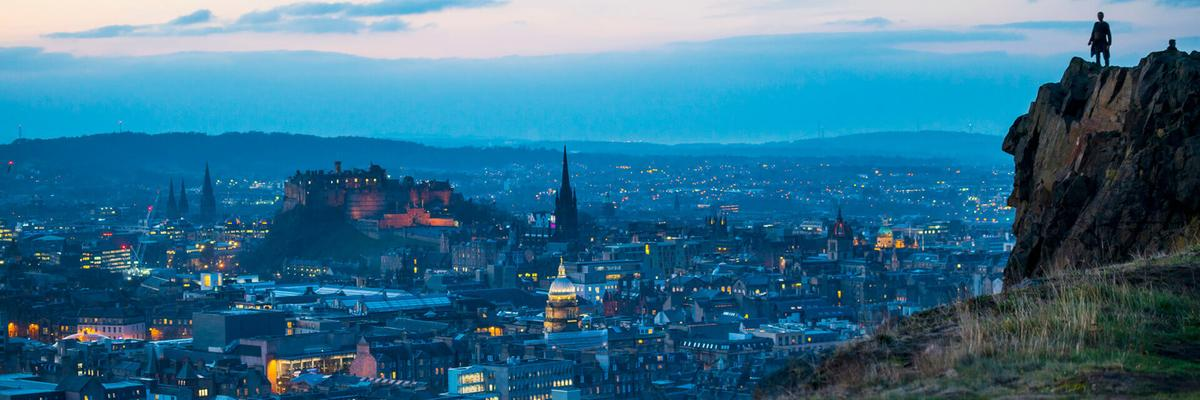
\includegraphics[width=1\textwidth,height=\textheight]{./images/edi.jpg}\\

\hypertarget{overview}{%
\section{Overview}\label{overview}}

After having the storm of Generative AI (Gen-AI), like ChatGPT, higher
education (HE) system started to discuss possibilities and challenges
since 2023. Whilst these tools provide transformative results, we must
ensure that students are using them critically for their teaching and
learning process. As mentioned in various reports and projections, as
higher education institutions, we should help them to be prepared for
work life after their study, but it is vital that those tools are used
as help rather than bypassing the learning process. There is an ongoing
debate on using such tools for teaching or not, with various strategies
or plans applied so far. The course level/content sensitivity is varying
with such tools, ie., proof-based mathematics vs.~programming modules.
Mainly, it is urgent to reconsider the teaching and learning under the
huge pressure of Gen-AI-based tools and their high-speed development.

As Gen-AI becomes widespread, it is crucial to provide an enriched
platform to share best practices and thought-provoking panel discussions
among the HE institutions. The proposed workshop aims to address this
critical challenge by bringing together a collection of educators and
teaching practitioners from related fields of study, especially
Mathematical Sciences / STEM.

We aim to stimulate discussions among teaching practitioners relying on
their experiences. The University of Edinburgh, in collaboration with
The University of Glasgow, will host this follow-up workshop to last
year's Glasgow event on rethinking assessment in times of Gen-AI,
keeping momentum going on interesting discussions.

\hypertarget{we-want}{%
\subsection{We want\ldots{}}\label{we-want}}

\ldots{} to foster the discussion alongside the recent Gen-AI related
improvements for the teaching and learning on mathematics education.
Possible themes are below but not limited to

\begin{itemize}
\tightlist
\item
  Integrating AI Tools in Mathematical Education
\item
  Ethical Considerations in AI-Driven Learning
\item
  Personalized Learning Pathways with AI
\item
  AI and the Evolution of Mathematical Problem Solving
\item
  Instructor Roles in an AI-Augmented Classroom
\item
  Assessing the Learning Outcomes in the Age of Gen-AI
\item
  How to develop Critical Thinking and AI Literacy
\end{itemize}

\begin{center}\rule{0.5\linewidth}{0.5pt}\end{center}

\hypertarget{workshop-details}{%
\section{Workshop Details}\label{workshop-details}}

\hypertarget{organisers}{%
\subsection{Organisers}\label{organisers}}

This event organized by,

\begin{itemize}
\tightlist
\item
  Ozan Evkaya (University of Edinburgh)
\item
  Jennifer Gaskel (University of Glasgow)
\item
  Skarleth Carrales Escobedo (University of Edinburgh)
\item
  Steven O'Hagan (University of Edinburgh)
\end{itemize}

For more details about this workshop, including registering your
interest, please contact:
\href{mailto:Ozan.Evkaya@ed.ac.uk}{\nolinkurl{Ozan.Evkaya@ed.ac.uk}}.

\hypertarget{where}{%
\subsection{Where?}\label{where}}

This workshop will be held in Edinburgh, hosted by the University of
Edinburgh

Venue:
\href{https://information-services.ed.ac.uk/computing/audio-visual-multi-media/teaching-spaces/interactive-360-degree-images-of-teaching-spaces/nucleus/nucleus-g02-elmlt}{Elm
Lecture Theatre}, Nucleus Building, The King's Buildings campus, The
University of Edinburgh, EH9 3FG

The Nucleus Building is a new shared learning, teaching and social hub
at the heart of The King's Buildings campus. See the location from the
\href{https://www.google.com/maps/place/The+Nucleus+Building,+The+University+of+Edinburgh/@55.9228707,-3.1739974,15z/data=!4m6!3m5!1s0x4887c74db76c8ddd:0x30d53c72c9accbd8!8m2!3d55.9229639!4d-3.1739935!16s\%2Fg\%2F11sb86zt46?entry=ttu\&g_ep=EgoyMDI1MDMzMS4wIKXMDSoJLDEwMjExNjQwSAFQAw\%3D\%3D}{Google
map}

\hypertarget{when}{%
\subsection{When?}\label{when}}

The event takes place on-site on \textbf{July 18, Friday, between
10.00-16.00}

\hypertarget{how-to-participate}{%
\subsection{How to participate?}\label{how-to-participate}}

Please reserve your seat until, \textbf{30th June 2025 Monday}. Please
note that capacity is limited, so registration may stop before the
deadline when all seats are taken!

See the \href{}{registration form} at your earliest convenience.

\hypertarget{tentative-schedule}{%
\subsection{Tentative Schedule}\label{tentative-schedule}}

\begin{longtable}[]{@{}
  >{\raggedright\arraybackslash}p{(\columnwidth - 2\tabcolsep) * \real{0.2252}}
  >{\raggedright\arraybackslash}p{(\columnwidth - 2\tabcolsep) * \real{0.7748}}@{}}
\toprule\noalign{}
\begin{minipage}[b]{\linewidth}\raggedright
\textbf{Time}
\end{minipage} & \begin{minipage}[b]{\linewidth}\raggedright
\textbf{Session Details}
\end{minipage} \\
\midrule\noalign{}
\endhead
\bottomrule\noalign{}
\endlastfoot
10:00 - 10:15 & Welcome and Introduction \\
10:15 - 11:00 & Main Speaker 1: Michael Grove -- TBA \\
11:00 - 11:30 & Lightning Talks Session 1 \\
11:30 - 12:00 & Tea/Coffee Break \\
12:00 - 12:45 & Main Speaker 2: Stuart King -- TBA \\
12:45 - 13:30 & Lunch Break (Will be served?) \\
13:45 - 14:00 & Discussion Topic 1 \\
14:00 - 14:30 & Lightning Talks Session 2 \\
14:30 - 14:45 & Tea/Coffee Break \\
14:45 - 15:00 & Discussion Topic 2 \\
15:00 - 15:45 & Main Speaker 3: TBA (Subject to funding) \\
\end{longtable}

15:45 - 16:00 \textbar{} Closing Remarks / Call for next year's Workshop
Series topic discussion \textbar{}

\hypertarget{keynote-speakers}{%
\subsection{KeyNote Speakers}\label{keynote-speakers}}

\hypertarget{michael-groove}{%
\subsubsection{\texorpdfstring{\href{https://www.birmingham.ac.uk/staff/profiles/maths/grove-michael}{Michael
Groove}}{Michael Groove}}\label{michael-groove}}

Michael Grove is Deputy Pro-Vice-Chancellor for Education Policy and
Academic Standards at the University of Birmingham, Professor of
Mathematics and Mathematics Education, and a National Teaching Fellow.

Talk Title and Abstract: TBA

\hypertarget{stuart-king}{%
\subsubsection{\texorpdfstring{\href{https://www.maths.ed.ac.uk/~sking3/index.html}{Stuart
King}}{Stuart King}}\label{stuart-king}}

He is working at the School of Mathematics at the University of
Edinburgh as a lecturer in Mathematics in 2015, as a member of the
Applied and Computational Mathematics research group.

Talk Title and Abstract: TBA

\hypertarget{speaker-3}{%
\subsubsection{\texorpdfstring{\href{}{Speaker
3}}{Speaker 3}}\label{speaker-3}}

Talk Title and Abstract: TBA

\begin{center}\rule{0.5\linewidth}{0.5pt}\end{center}

\hypertarget{higher-education-teaching-and-learning-series-2025}{%
\section{Higher Education Teaching and Learning Series
2025}\label{higher-education-teaching-and-learning-series-2025}}

\hypertarget{other-events}{%
\subsection{Other events?}\label{other-events}}

Please see the other events happening this year below;

\begin{longtable}[]{@{}
  >{\raggedright\arraybackslash}p{(\columnwidth - 4\tabcolsep) * \real{0.1250}}
  >{\raggedright\arraybackslash}p{(\columnwidth - 4\tabcolsep) * \real{0.6488}}
  >{\raggedright\arraybackslash}p{(\columnwidth - 4\tabcolsep) * \real{0.2262}}@{}}
\toprule\noalign{}
\begin{minipage}[b]{\linewidth}\raggedright
\textbf{Date}
\end{minipage} & \begin{minipage}[b]{\linewidth}\raggedright
\textbf{Event Title}
\end{minipage} & \begin{minipage}[b]{\linewidth}\raggedright
\textbf{Institution}
\end{minipage} \\
\midrule\noalign{}
\endhead
\bottomrule\noalign{}
\endlastfoot
\textbf{12 JUNE} & \emph{Fostering Engagement and Learning in
Mathematics in the Digital Age} & University of Central Lancashire \\
\textbf{4 JULY} & \emph{Rethinking feedback and assessment: what does
this mean in traditionally exam-based mathematics?} & Imperial College
London \\
\textbf{10 JULY} & \emph{Enhancing Student Community and Learning:
Adapting Strategies for Changing Patterns of Student Engagement} & The
Open University \\
\textbf{?? JULY} & \emph{Automatic grading in mathematics and
statistics: beyond the basics} & University of Liverpool \\
\end{longtable}

\begin{center}\rule{0.5\linewidth}{0.5pt}\end{center}

\hypertarget{speaker-slides}{%
\section{Speaker Slides}\label{speaker-slides}}

Please see the keynote speaker slides and participant contributions from
that list

\hypertarget{keynote}{%
\subsection{KeyNote}\label{keynote}}

\begin{itemize}
\tightlist
\item
  \href{}{Michael Groove}
\item
  \href{}{Stuart King}
\item
  \href{}{Speaker 3}
\end{itemize}

\hypertarget{lightning-talks}{%
\subsection{Lightning Talks}\label{lightning-talks}}

\begin{itemize}
\tightlist
\item
  \href{}{Lightning Talk Speaker 1}
\end{itemize}

\hypertarget{feedback-and-further-suggestions}{%
\section{Feedback and Further
suggestions}\label{feedback-and-further-suggestions}}

Thank you for your participation! Please give us feedback regarding the
workshop event and your further suggestions!

\begin{itemize}
\tightlist
\item
  \href{}{Participation Survey}
\end{itemize}

\begin{center}\rule{0.5\linewidth}{0.5pt}\end{center}

This workshop event is mainly funded and supported by;

\begin{figure}

\begin{minipage}[t]{0.50\linewidth}

{\centering 


\includegraphics[width=0.75\textwidth,height=\textheight]{./images/IMA_logo.png}\\

}

\end{minipage}%
%
\begin{minipage}[t]{0.50\linewidth}

{\centering 


\includegraphics[width=0.75\textwidth,height=\textheight]{./images/LMS_logo.png}\\

}

\end{minipage}%

\end{figure}

\begin{figure}

\begin{minipage}[t]{0.50\linewidth}

{\centering 


\includegraphics[width=0.75\textwidth,height=\textheight]{./images/RSS.png}\\

}

\end{minipage}%
%
\begin{minipage}[t]{0.50\linewidth}

{\centering 


\includegraphics[width=0.75\textwidth,height=\textheight]{./images/GAIL_logo.jpg}\\

}

\end{minipage}%

\end{figure}



\end{document}
